% Sección 9. Responsable: Juan Diego (#46).
% Cifras: outputs/modelado/comparacion/ (scripts/modelado/comparacion.py), que recalcula cada
% métrica desde las predicciones guardadas por #42 a #45 y #144 y la coteja con el CSV de su issue.
% Los modelos finales son los ajustados en #45 (outputs/modelado/ajuste/) y la regresión de #144 (outputs/modelado/regresion/).
\section{Resultados}\label{sec:resultados}

Esta sección compara los cinco modelos ajustados, SARIMA, ETS, regresión lineal, bosque aleatorio y potenciación del gradiente por histogramas, con la barra de D-04: el ingenuo estacional, con un MAE de 49,04 en el conjunto de evaluación (sección~\ref{sec:barra}). Sus configuraciones se eligieron con los seis pliegues de origen rodante, sin usar los 184 días de evaluación (tabla~\ref{tab:busqueda} del apéndice). La evaluación final se calculó una sola vez, después de la selección. Toda cifra de esta sección sale de \texttt{outputs/\allowbreak{}modelado/\allowbreak{}comparacion/}. El script que la produce recalcula cada métrica desde las predicciones guardadas y se detiene si alguna no coincide con la tabla de su issue. Así se cotejaron 616 cifras.

\subsection{Comparación con la barra}\label{sec:res-barra}

Los cinco modelos bajan el MAE de la barra: SARIMA, ETS y los dos árboles entre un 30 y un 33\,\%, y la regresión lineal un 26\,\% (tabla~\ref{tab:resultados}). También mejoran el RMSE y el MAPE, y los cinco quedan con un MASE de entre 0,615 y 0,683. Es decir, su error es entre un 32 y un 38\,\% menor que el del ingenuo estacional dentro del propio entrenamiento, que es la referencia del MASE.

Para saber si la diferencia con la barra es mayor que el azar de una sola ventana de evaluación se usa la prueba de \citet{diebold1995}. La prueba compara, día a día, la pérdida de los dos pronósticos. Se aplica con la corrección para muestras pequeñas de \citet{harvey1997} y con pérdida absoluta, coherente con el MAE. En SARIMA, ETS y los árboles el valor $p$ es menor que $10^{-7}$, y en la regresión lineal es de $7\times10^{-6}$. El resultado se mantiene con pérdida cuadrática y con la varianza de \citet{newey1987} con 7 rezagos, que tiene en cuenta que los errores de días consecutivos están correlacionados. Ningún comparador trivial se distingue de la barra salvo la media móvil de 28 días, que es peor ($p = 0{,}048$).

\begin{table}[H]
\centering
\caption{Modelos ajustados y comparadores triviales en el conjunto de evaluación (184 días, del 2025-05-01 al 2025-10-31). $\Delta$MAE: diferencia relativa con la barra. $p$: prueba de Diebold-Mariano contra la barra (pérdida absoluta, corrección de Harvey, Leybourne y Newbold). Fuente: \texttt{outputs/\allowbreak{}modelado/\allowbreak{}comparacion/\allowbreak{}tabla\_\allowbreak{}comparativa.csv}.}\label{tab:resultados}
\small
\begin{tabular}{@{}lrrrrrr@{}}
\toprule
\textbf{Modelo} & \textbf{MAE} & \textbf{RMSE} & \textbf{MAPE} & \textbf{MASE} & \textbf{$\Delta$MAE} & \textbf{$p$} \\
\midrule
Gradiente por histogramas & 32,72 & 42,39 & 9,68\,\% & 0,615 & $-$33,3\,\% & $2\times10^{-9}$ \\
ETS & 32,95 & 42,21 & 9,50\,\% & 0,619 & $-$32,8\,\% & $2\times10^{-9}$ \\
SARIMA & 33,57 & 42,97 & 9,80\,\% & 0,631 & $-$31,5\,\% & $1\times10^{-9}$ \\
Bosque aleatorio & 34,22 & 42,69 & 9,86\,\% & 0,643 & $-$30,2\,\% & $2\times10^{-8}$ \\
Regresión lineal & 36,31 & 46,54 & 10,47\,\% & 0,683 & $-$26,0\,\% & $7\times10^{-6}$ \\
\midrule
\textbf{Ingenuo estacional (barra)} & \textbf{49,04} & \textbf{61,44} & \textbf{14,39\,\%} & \textbf{0,922} & --- & --- \\
Media móvil de 7 días & 49,42 & 61,86 & 14,59\,\% & 0,929 & 0,8\,\% & 0,91 \\
Ingenuo & 52,92 & 68,41 & 15,62\,\% & 0,995 & 7,9\,\% & 0,35 \\
Media móvil de 28 días & 55,83 & 70,72 & 16,75\,\% & 1,050 & 13,8\,\% & 0,048 \\
\bottomrule
\end{tabular}
\end{table}

\subsection{Estabilidad entre pliegues}\label{sec:res-estabilidad}

Batir la barra en una sola ventana no basta, porque el orden de los comparadores cambia con la ventana (sección~\ref{sec:barra}). La tabla~\ref{tab:estabilidad} repite la comparación en los seis pliegues, contra el mismo comparador. Los cinco modelos ganan al ingenuo estacional en los seis. Además varían mucho menos: la desviación de su MAE entre pliegues va de 4,34 a 7,46, y la del ingenuo estacional es de 14,11. El peor pliegue de cada modelo, entre 35,49 y 44,61, queda muy por debajo del peor de la barra, 75,57.

La figura~\ref{fig:mae-pliegue} muestra que los modelos y la barra coinciden en qué ventanas son más fáciles: los pliegues 3 y 4, de mayo a noviembre de 2024. En los pliegues difíciles, la barra empeora mucho más que los modelos. El gradiente por histogramas tiene el menor MAE medio en los pliegues (30,82) y la menor desviación (4,34). Ese MAE medio es el criterio con el que se eligió su configuración, así que no es una medida independiente. La regresión lineal tiene el segundo menor MAE medio (34,57), por delante de SARIMA y ETS, aunque en la evaluación final es la de mayor error. El orden en los pliegues tampoco anticipa el de la evaluación final.

\begin{table}[H]
\centering
\caption{MAE en los seis pliegues de origen rodante. Pliegues ganados: aquellos en los que el modelo tiene menor MAE que el ingenuo estacional. Fuente: \texttt{outputs/\allowbreak{}modelado/\allowbreak{}comparacion/\allowbreak{}tabla\_\allowbreak{}comparativa.csv} y \texttt{mae\_\allowbreak{}por\_\allowbreak{}pliegue.csv}.}\label{tab:estabilidad}
\small
\begin{tabular}{@{}lrrrr@{}}
\toprule
\textbf{Modelo} & \textbf{MAE medio} & \textbf{Desviación} & \begin{tabular}[b]{@{}r@{}}\textbf{Peor}\\\textbf{pliegue}\end{tabular} & \begin{tabular}[b]{@{}r@{}}\textbf{Pliegues}\\\textbf{ganados}\end{tabular} \\
\midrule
Gradiente por histogramas & 30,82 & 4,34 & 35,49 & 6 de 6 \\
Regresión lineal & 34,57 & 5,02 & 41,27 & 6 de 6 \\
Bosque aleatorio & 34,89 & 7,46 & 43,12 & 6 de 6 \\
ETS & 36,04 & 5,89 & 44,61 & 6 de 6 \\
SARIMA & 36,11 & 5,60 & 42,58 & 6 de 6 \\
\midrule
Ingenuo estacional (barra) & 58,30 & 14,11 & 75,57 & --- \\
Ingenuo & 58,36 & 9,37 & 75,48 & 4 de 6 \\
\bottomrule
\end{tabular}
\end{table}

\begin{figure}[H]
\centering
\IfFileExists{figuras/modelos_mae_por_pliegue.pdf}{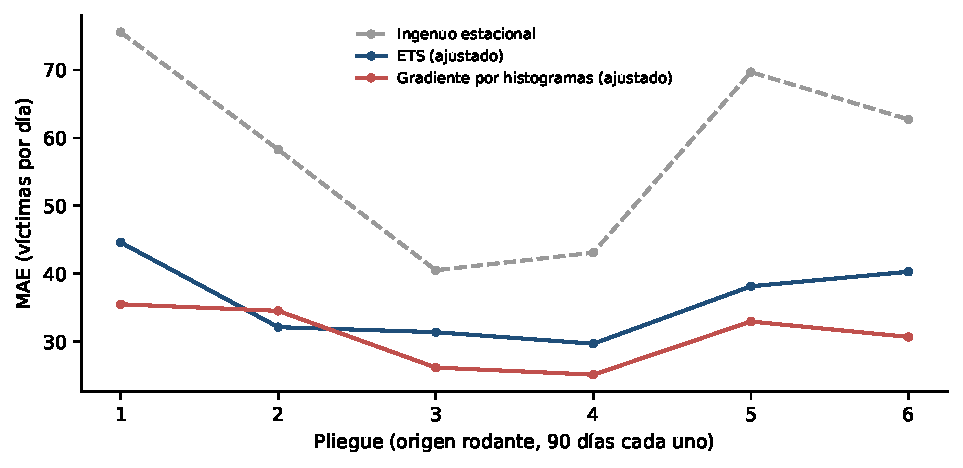
\includegraphics[width=0.8\textwidth]{figuras/modelos_mae_por_pliegue.pdf}}{\fbox{Figura pendiente: \texttt{figuras/modelos\_mae\_por\_pliegue.pdf}}}
\caption{MAE por pliegue del ingenuo estacional y de los modelos con menor MAE medio en los pliegues de cada familia. Fuente: \texttt{outputs/\allowbreak{}modelado/\allowbreak{}comparacion/\allowbreak{}mae\_\allowbreak{}por\_\allowbreak{}pliegue.csv}.}\label{fig:mae-pliegue}
\end{figure}

\subsection{Diferencias entre los modelos}\label{sec:res-entre-modelos}

Entre SARIMA, ETS y los dos árboles, la diferencia entre el mejor y el peor es de 1,50 víctimas por día de MAE, y la prueba de Diebold-Mariano no encuentra ninguna diferencia significativa entre ellos: los valores $p$ van de 0,17 a 0,91 (tabla~\ref{tab:dm-pares}). La regresión lineal queda entre 2,09 y 3,59 víctimas por encima de esos cuatro. Solo la diferencia con el gradiente es significativa al 5\,\% ($p = 0{,}023$), y deja de serlo con la varianza de \citet{newey1987}, que tiene en cuenta la autocorrelación de los errores ($p = 0{,}073$). Además, son diez comparaciones sin corrección por multiplicidad. Con estos 184 días no hay un ganador entre los cuatro mejores modelos, y la regresión es la más débil sin que eso se pueda afirmar con solidez. Lo que sí se sostiene es que los cinco superan la barra y que lo hacen en todos los pliegues.

\begin{table}[H]
\centering
\caption{Prueba de Diebold-Mariano entre pares de modelos ajustados en el conjunto de evaluación (pérdida absoluta). $p$ (HLN): con la corrección de Harvey, Leybourne y Newbold. $p$ (NW): con la varianza de Newey-West con 7 rezagos. Fuente: \texttt{outputs/\allowbreak{}modelado/\allowbreak{}comparacion/\allowbreak{}diebold\_\allowbreak{}mariano\_\allowbreak{}entre\_\allowbreak{}modelos.csv}.}\label{tab:dm-pares}
\small
\begin{tabular}{@{}llrrr@{}}
\toprule
\textbf{Modelo A} & \textbf{Modelo B} & \textbf{MAE A -- MAE B} & \textbf{$p$ (HLN)} & \textbf{$p$ (NW)} \\
\midrule
Gradiente por histogramas & ETS & $-$0,23 & 0,91 & 0,94 \\
Gradiente por histogramas & SARIMA & $-$0,85 & 0,65 & 0,73 \\
Gradiente por histogramas & Bosque aleatorio & $-$1,50 & 0,17 & 0,14 \\
ETS & SARIMA & $-$0,62 & 0,49 & 0,51 \\
ETS & Bosque aleatorio & $-$1,27 & 0,47 & 0,55 \\
SARIMA & Bosque aleatorio & $-$0,65 & 0,68 & 0,72 \\
\midrule
Gradiente por histogramas & Regresión lineal & $-$3,59 & 0,023 & 0,073 \\
ETS & Regresión lineal & $-$3,36 & 0,12 & 0,19 \\
SARIMA & Regresión lineal & $-$2,74 & 0,16 & 0,22 \\
Bosque aleatorio & Regresión lineal & $-$2,09 & 0,18 & 0,23 \\
\bottomrule
\end{tabular}
\end{table}

\subsection{Pronóstico frente a observado y errores por periodo}\label{sec:res-periodos}

La figura~\ref{fig:pronostico} superpone, para los 184 días de evaluación, lo observado, la barra y el modelo con menor MAE medio en los pliegues de cada familia: ETS, el gradiente y la regresión lineal. Los tres siguen el ciclo semanal. La barra, en cambio, repite con una semana de retraso los días anómalos, como se ve en los picos y caídas aislados de la línea discontinua.

\begin{figure}[H]
\centering
\IfFileExists{figuras/modelos_pronostico_observado.pdf}{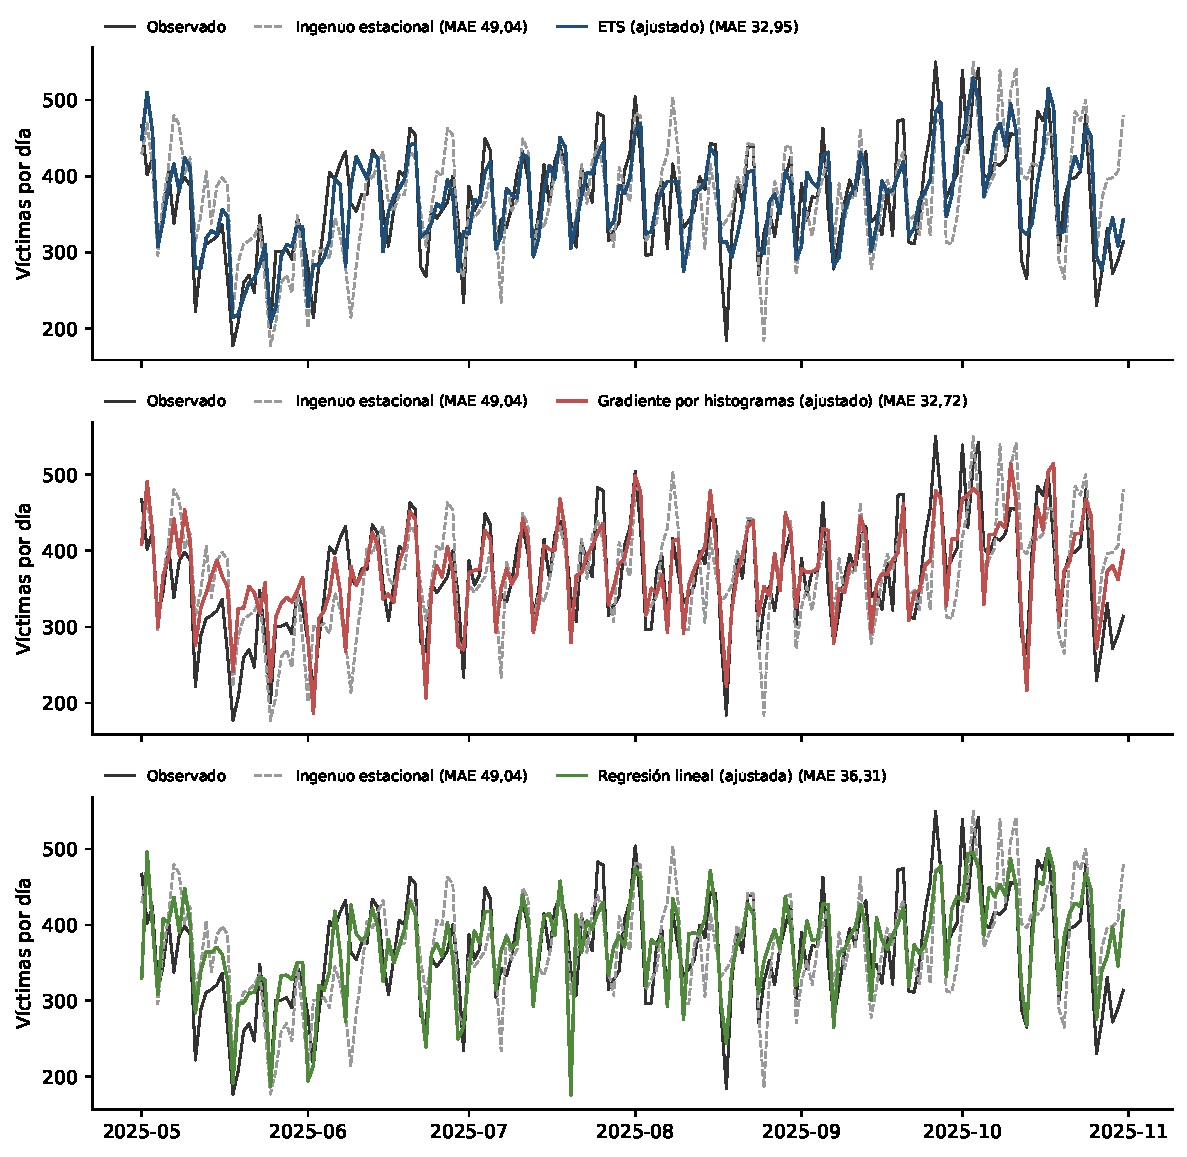
\includegraphics[width=\textwidth]{figuras/modelos_pronostico_observado.pdf}}{\fbox{Figura pendiente: \texttt{figuras/modelos\_pronostico\_observado.pdf}}}
\caption{Víctimas diarias observadas y pronosticadas un día adelante en el conjunto de evaluación. Arriba, ETS; en medio, gradiente por histogramas; abajo, regresión lineal; en gris, el ingenuo estacional. Fuente: \texttt{outputs/\allowbreak{}modelado/\allowbreak{}comparacion/}.}\label{fig:pronostico}
\end{figure}

\textbf{Los festivos separan a los modelos que ven el calendario de los que no.} En los ocho festivos del conjunto de evaluación, SARIMA y ETS se equivocan en 72,41 y 68,81 víctimas de media, y sobrestiman en 58,73 y 55,67 (tabla~\ref{tab:festivos}). Su error en un festivo es casi tan grande como el de la barra. Estos modelos solo ven la propia serie, sin variables de calendario. Por eso pronostican el festivo como un día normal de su día de la semana. Los árboles, que sí tienen la variable de festivo, bajan ese error a 36,68 y 42,73, aunque tienden a subestimar. La regresión lineal, con las mismas variables de calendario, queda en medio, con 54,51, y también subestima (sesgo de $-$30,70). En los días que no son festivos, los cinco modelos quedan entre 31,32 y 35,48. Ocho días son pocos para estimar con precisión, pero la dirección coincide con el análisis exploratorio: un lunes festivo registra un 38\,\% menos de víctimas que uno laborable (sección~\ref{sec:eda-semana}). Es el primer candidato para mejorar los modelos de series, por ejemplo con el festivo como variable exógena.

\begin{table}[H]
\centering
\caption{Error absoluto medio y sesgo (pronóstico menos observado) según el tipo de día, en el conjunto de evaluación. Fuente: \texttt{outputs/\allowbreak{}modelado/\allowbreak{}comparacion/\allowbreak{}errores\_\allowbreak{}por\_\allowbreak{}periodo.csv}.}\label{tab:festivos}
\small
\begin{tabular}{@{}lrrrr@{}}
\toprule
& \multicolumn{2}{c}{\textbf{Festivos (8 días)}} & \multicolumn{2}{c}{\textbf{No festivos (176 días)}} \\
\cmidrule(lr){2-3}\cmidrule(l){4-5}
\textbf{Modelo} & \textbf{MAE} & \textbf{Sesgo} & \textbf{MAE} & \textbf{Sesgo} \\
\midrule
Gradiente por histogramas & 42,73 & $-$24,34 & 32,26 & 9,78 \\
Bosque aleatorio & 36,68 & $-$11,76 & 34,11 & 2,93 \\
Regresión lineal & 54,51 & $-$30,70 & 35,48 & 10,55 \\
ETS & 68,81 & 55,67 & 31,32 & $-$0,49 \\
SARIMA & 72,41 & 58,73 & 31,81 & $-$0,76 \\
\midrule
Ingenuo estacional (barra) & 80,38 & 63,38 & 47,61 & 1,66 \\
\bottomrule
\end{tabular}
\end{table}

\textbf{Por mes,} octubre es difícil para todos los modelos, con un MAE de entre 37,83 y 42,43, y también para la barra (66,03). En mayo los modelos se separan: los árboles y la regresión sobrestiman (sesgo de 39,81 en el gradiente, 30,24 en el bosque y 28,51 en la regresión, con MAE de 47,38, 42,25 y 42,23), mientras SARIMA y ETS quedan en 29,65 y 27,05. Para el gradiente y la regresión, mayo es el peor mes. Por día de la semana no aparece un patrón común a los cinco modelos. El dato completo por mes y por día está en \texttt{errores\_\allowbreak{}por\_\allowbreak{}periodo.csv}.

\textbf{No hay análisis de error por localidad.} La serie que se modela es la de toda la ciudad, porque el registro de la Policía no identifica la localidad (D-01, sección~\ref{sec:limitaciones-metodo}). Ningún modelo produce un pronóstico por localidad, así que no hay errores territoriales que medir.

\subsection{Sensibilidad a 2020}\label{sec:res-sensibilidad}

D-04 exige comprobar qué pasa sin 2020. Los árboles y la regresión se reentrenan sin las filas de ese año, y SARIMA y ETS, desde el 2021-01-01. Con la configuración elegida en cada caso, el MAE final cambia entre $-$0,57 (gradiente, 32,15) y $+$0,79 (regresión, 37,10). Las cinco variantes siguen ganando a la barra en los seis pliegues, con $p < 10^{-8}$ en SARIMA, ETS y los árboles y $p = 3\times10^{-5}$ en la regresión (\texttt{tabla\_\allowbreak{}comparativa.csv}). Ninguna conclusión de esta sección depende de cómo se trate 2020.
